\documentclass[letterpaper, 10 pt, conference]{ieeeconf}  
\usepackage[utf8]{inputenc} % allow utf-8 input
\usepackage[T1]{fontenc}    % use 8-bit T1 fonts
\usepackage{subfigure}		% For subfigures
\usepackage{microtype}      % microtypography
\usepackage{graphicx}       % microtypography
\usepackage{amsfonts}       % blackboard math symbols
\usepackage{booktabs}       % professional-quality tables
\usepackage{nicefrac}       % compact symbols for 1/2, etc.
\usepackage{breqn}          % dmath multiline
\usepackage{url}            % simple URL typesetting
\usepackage[backend=bibtex,style=ieee,mincitenames=1,maxcitenames=2,maxbibnames=20]{biblatex}
\addbibresource{paper.bib}

\usepackage[keeplastbox]{flushend}

\IEEEoverridecommandlockouts
\overrideIEEEmargins
\title{\LARGE \bf World Models for Deep Reinforcement Learning}
\author{Shawn Manuel$^{1}$ and Mykel J. Kochenderfer$^{2}$
\thanks{$^{1}$Shawn Manuel is with the Department of Computer Science at Stanford University, Stanford, CA. Email: {\tt\small sman64@stanford.edu}}%
\thanks{$^{2}$Mykel J. Kochenderfer is with the Department of Aeronautics and Astronautics at Stanford University, Stanford, CA. Email: {\tt\small mykel@stanford.edu}}%
}

\begin{document}

\maketitle
\thispagestyle{empty}
\pagestyle{empty}

\begin{abstract}

We consider an application of the recently successful `World Model' architecture using generative neural networks in reinforcement learning to abstract high dimensional image observations into compressed spatial and temporal vector representation. We propose to incorporate the World Model with a deep reinforcement learning agent to learn an action-selection policy from the high-level features of the environment represented by the World Model. We tested two policy gradient actor-critic learning algorithms, Deep Deterministic Policy Gradients and Proximal Policy Optimization, trained using the World Model on OpenAI Gym's CarRacing-v0. We found that these agents were able to achieve scores at the level of the current state of the art evolutionary algorithms for training an agent. It was also observed that the simplified state representation of the World Model improved the speed and stability of the training process as well as enabling simpler neural network architectures than equivalent agents trained from raw image states.
	
\end{abstract}
\section{INTRODUCTION}

Deep Reinforcement Learning is a growing field where neural networks are employed to learn a general policy for selecting actions in a given environment. State of the art reinforcement learning algorithms such as Q-Learning have evolved to allow neural networks to learn effective policies for simple control tasks such as balancing a cartpole or swinging a pendulum. In these cases, the agent often has access to the true dynamics of the environment as a low dimensional observation and is therefore able to learn optimal policies using a simple feed forward neural network. However, tasks such as learning to control a simulated car and then navigate a track given only raw images are much more difficult to learn with standard Deep Q-Learning algorithms. Furthermore, as dynamic information such as velocity and acceleration cannot be inferred from a single image, requiring the agent to either train an RNN to store the state history or receive input of stacked image frames to translate to optimal actions to select. This increases the computational load on deep RL where it has to learn a representation of the temporal structure in addition to learning the optimal policy. Therefore, this leads to the motivation to decouple the reinforcement learning task into (1) environment simplification, and (2) optimal action selection.

The task of learning an optimal policy from high dimensional images has many practical applications in real-life situations where the true dynamics are often unknown. Autonomous driving using computer vision control systems is a growing area of study where sensory data is often in image form \cite{4.0}. For these tasks, the ability to learn a stable control policy for safely driving a vehicle is a challenging optimization problem for deep reinforcement learning agents using large convolutional layers to process these images. Robotics is another application where deep reinforcement learning agents have been applied to train a robot arm to manipulate objects on a table from visual observations \cite{5.0}. This often requires thousands of training episodes to adequately learn the task, where the agent's representation of the environment may not even be transferable to other similar tasks. Since the latent features of a state space are generally constant, there is potential to improve training efficiency with offline learning of a mapping from high-dimensional images to a simplified environment state space, then using this model to compress the visual observation into a smaller dimensional input to train a policy via reinforcement learning. By modeling the environment separately, the learned model can be transferred to other agents learning different tasks from the same environment observations.

Previous approaches to addressing this problem have use a convolutional neural network to compress the state to latent vector and then have a separate RNN to learn the temporal history, however, the representation of the dynamics is coupled with the policy learned. As a result, using the trained convolutional network and RNN to train a new policy from scratch would introduce irrelevant features for a policy to learn from without retraining the CNN and RNN when learning. Ha and Schmidhuber \cite{1.0.0} recently introduced the ``World Models'' architecture which decouples of the environment representation from policy learning. This involved a visual module that maps high dimensional images to a lower dimensional code, a memory module that modeled temporal dynamics of the environment, and a simple decision-making module that determines the action an agent should take based on the compressed visual and temporal representations. Using Covariance-Matrix Adaptation evolutionary strategy (CMA) \cite{1.0.3} to train the decision-making module, this system achieved a new state of the art performance for a challenging simulated car racing environment with purely visual observations. However, CMA requires many iterations to search for a policy and is also only effective when the parameter space is small. Using RL algorithms to train using the world model is an unexplored approach for efficiently learning a policy for a model with more parameters. In this paper, we incorporate the World Model architecture to simplify the dimensionality of the image observations received from the environment to allow a reinforcement learning agent to focus on maximizing reward using the relevant features of the environment observations. We then evaluate the performance of such agents relative to the agent in \cite{1.0.0} on the same car racing environment. Our approach achieves state of the art performance on this environment without requiring any domain-specific modifications to the environment outputs.

This report will be structured as follows: Section \ref{background} provides a background to the field of reinforcement learning and the car racing environment as well as previous approaches to solve it; Section \ref{approach} outlines the architecture and approach for training the reinforcement agents using the World Model; and Section \ref{experiments} provides an experimental evaluation of the agents trained.


% The challenge here is that in environments with high dimensional non-markov state inputs (like pixels) the RL algorithm either needs to train an RNN to store the state history or receive input of stacked image frames. This increases the computational load on deep RL where it has to learn a representation of the temporal structure in addition to learning the optimal policy. Even when a representation is learned, this isn’t transferrable to other policies learning with the same environment dynamics.

% Why is it interesting and important? It is beneficial to learn a latent model of the high dimensional state space separate from training a policy because the environment dynamics are generally constant, so it is redundant for different policies trained from scratch on the same environment to have to learn this representation each time. Offline learning of a simplified environment state space is particularly applicable in robotics or self driving cars where the latent features of a state space are generally constant, but different tasks will require different policies, hence the learning of the state representation can be separated from learning the policy.

% Why is it hard? The naive approach is to use a convolutional neural network to compress the state to latent vector and then have a separate RNN to learn the temporal history however the representation of the dynamics is coupled with the policy learned, so using the trained convolutional network and RNN to train a new policy from scratch would introduce irrelevant features for a policy to learn from without retraining the CNN and RNN when learning (which would essentially be training from scratch)

% Why hasn’t it been solved before? Previous approaches to addressing this problem have used the method described in 3., however a recent paper “World Models” introduced this decoupling of the environment representation to policy where the policy is trained by CMA evolution. However, CMA requires many iterations to search for a policy and is also only effective when the parameter space is small. Using RL algorithms to train using the world model is an unexplored approach for efficiently learning a policy for a model with more parameters.

% What are the key components? Key components include using Deep RL algorithms such as PPO and DDPG in place of CMA to speed up training. This is evaluated on the CarRacing-v0 environment on OpenAI gym and compared to other papers solving that environment, my approach achieves state of the art performance (100 episode average reward of 900+ for both DDPG and PPO) whereas other attempts have achieved a maximum of 600 and others also require discretization of the continuous action space using domain knowledge. My approach doesn’t require any modifications to the environment outputs.
\section{BACKGROUND}\label{background}

We consider the standard partially observable reinforcement learning setting where an agent interacts with an environment $\mathcal{E}$ receiving image observations which do not contain temporal information~\cite{arulkumaran2017brief}. At each time step $t$, the agent receives an observation $s_t$ and selects an action $a_t$ according to a policy $\pi$, which is a mapping from observations to actions. The agent then receives a next observation $s_{t+1}$, a scalar reward $r_t \in \mathbb{R}$, and a Boolean flag $d_t$ indicating whether the agent reached a terminal state. An experience tuple at time $t$ is $(s_t, a_t, s_{t+1}, r_t, d_t)$. A sequence of experience tuples from an initial state to a terminal state is known as a trajectory. The goal of an RL agent is to maximize the total expected cumulative reward at each time step, defined as $R_t = \sum_{k=0}^{\infty} \gamma^{k}r_{t+k}$ for a discount rate $\gamma \in (0,1]$~\cite{mnih2016asynchronous}.

\subsection{Visual-based RL Environments}

The three environments explored in this paper are OpenAI Gym's \texttt{CarRacing-v0}, and the \texttt{take\_cover} and \texttt{defend\_the\_line} scenarios from the ViZDoom platform.

\begin{figure}[h!]
	\centering
	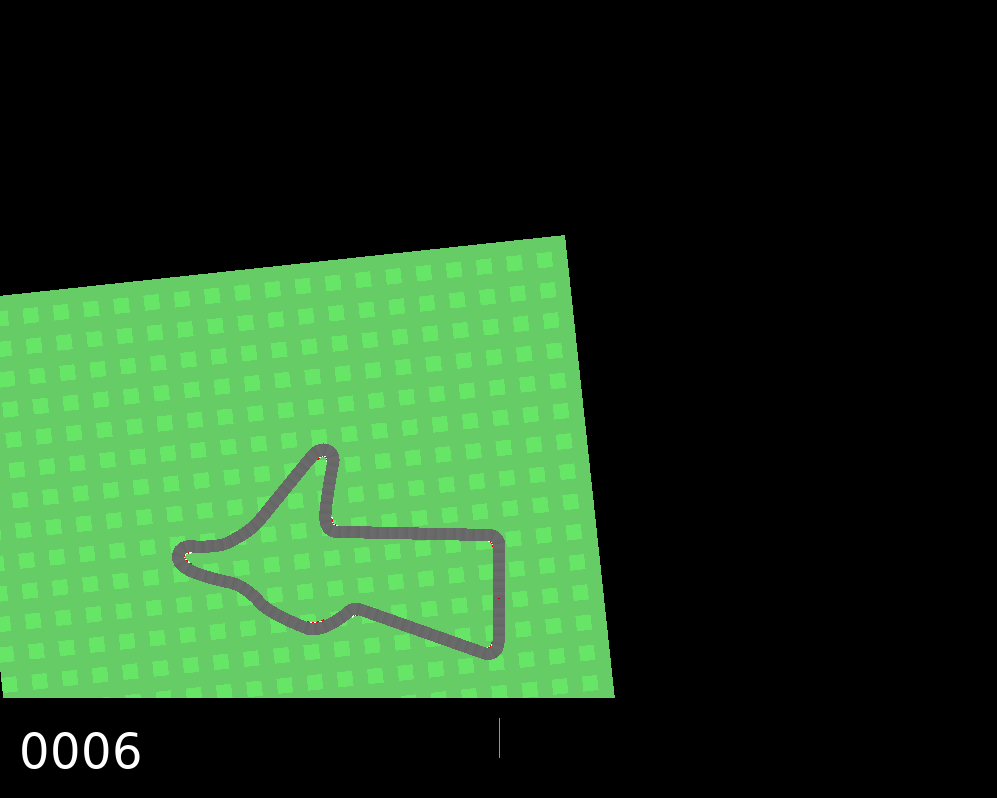
\includegraphics[width=0.15\textwidth]{images/car-map.png}
	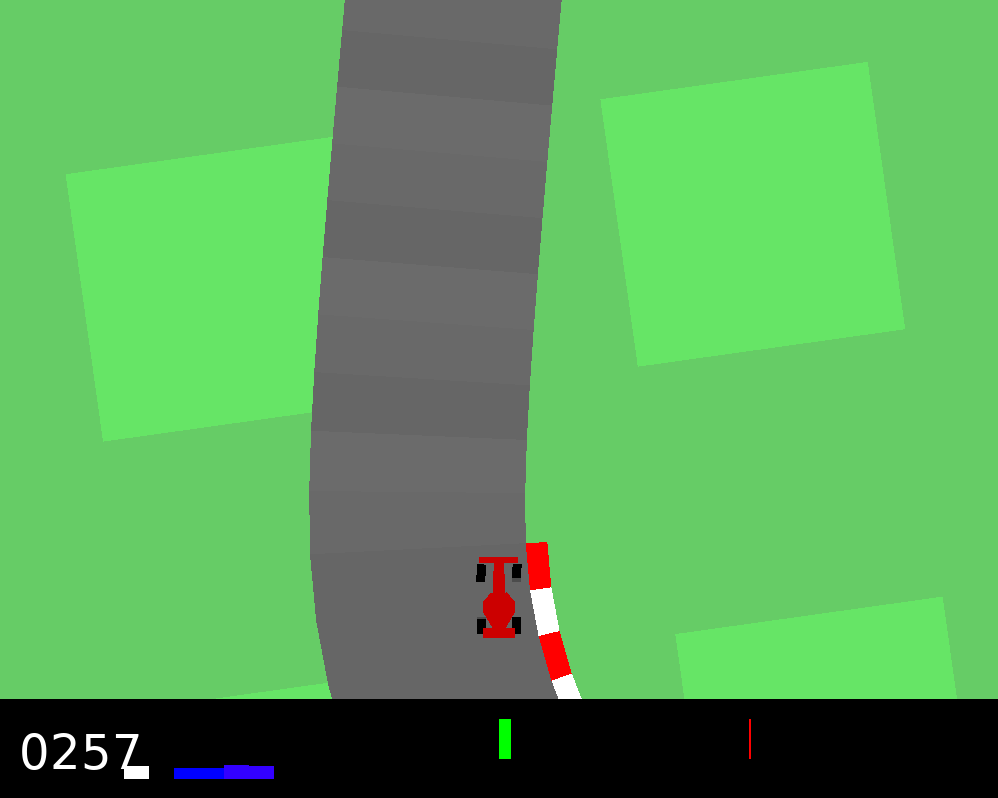
\includegraphics[width=0.15\textwidth]{images/car-tile.png}
	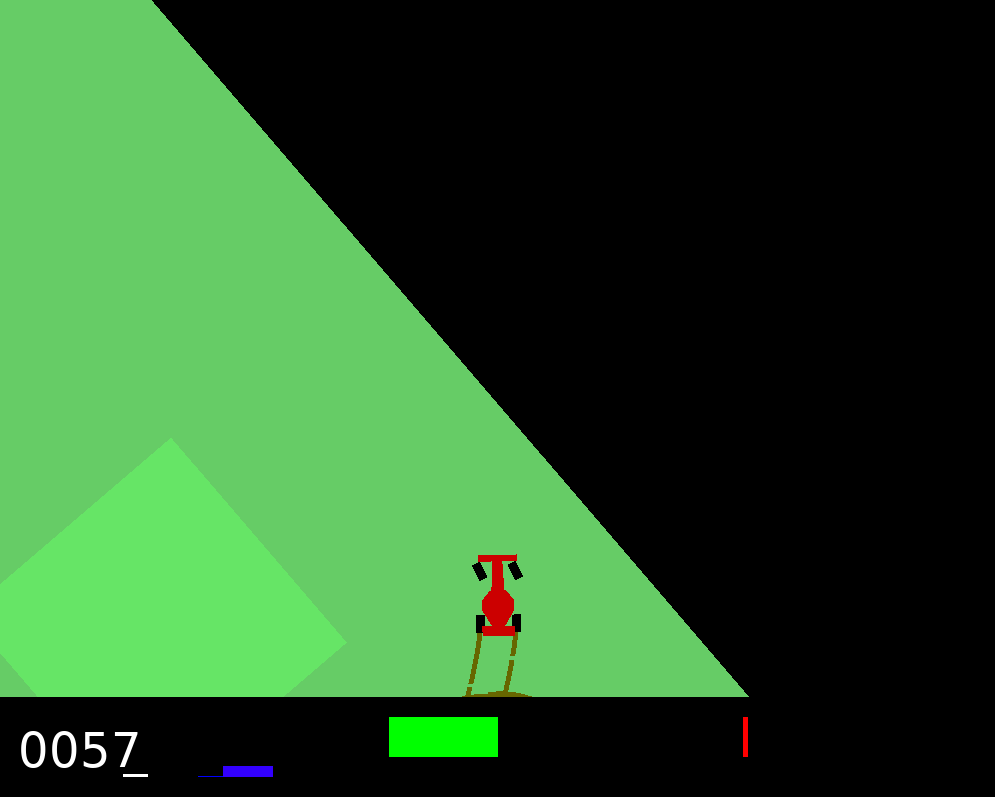
\includegraphics[width=0.15\textwidth]{images/car-die.png}
	\caption{Random Map (left), State Image (middle), Edge of map (right)}\label{fig:carracing}
\end{figure}

\subsubsection{CarRacing-v0}

The \texttt{CarRacing-v0} environment on OpenAI Gym~\cite{brockman2016openai} is a continuous action-space environment where the goal is to control the steering, acceleration, and braking of a car to race it around a randomly generated circuit track in as few time steps as possible. Each observation is an image of the top view of the car on the map as shown in \cref{fig:carracing}. The agent then needs to provide an action consisting of three continuous values for the steering, acceleration, and brake. The track is overlaid with $n$ (usually between $230$ and $320$) rectangular tiles shown in \cref{fig:carracing} (middle) where the agent receives a reward of $1000/n$ upon visiting a tile for the first time. A trajectory terminates after $1000$ time steps, after the agent visits every tile, or after the agent drives off the edge of the map (right of \cref{fig:carracing}). The agent also receives a penalty of $-0.1$ at each time step, encouraging faster completion of the circuit.

\subsubsection{take\_cover and defend\_the\_line}

\begin{figure}[h!]
	\centering
	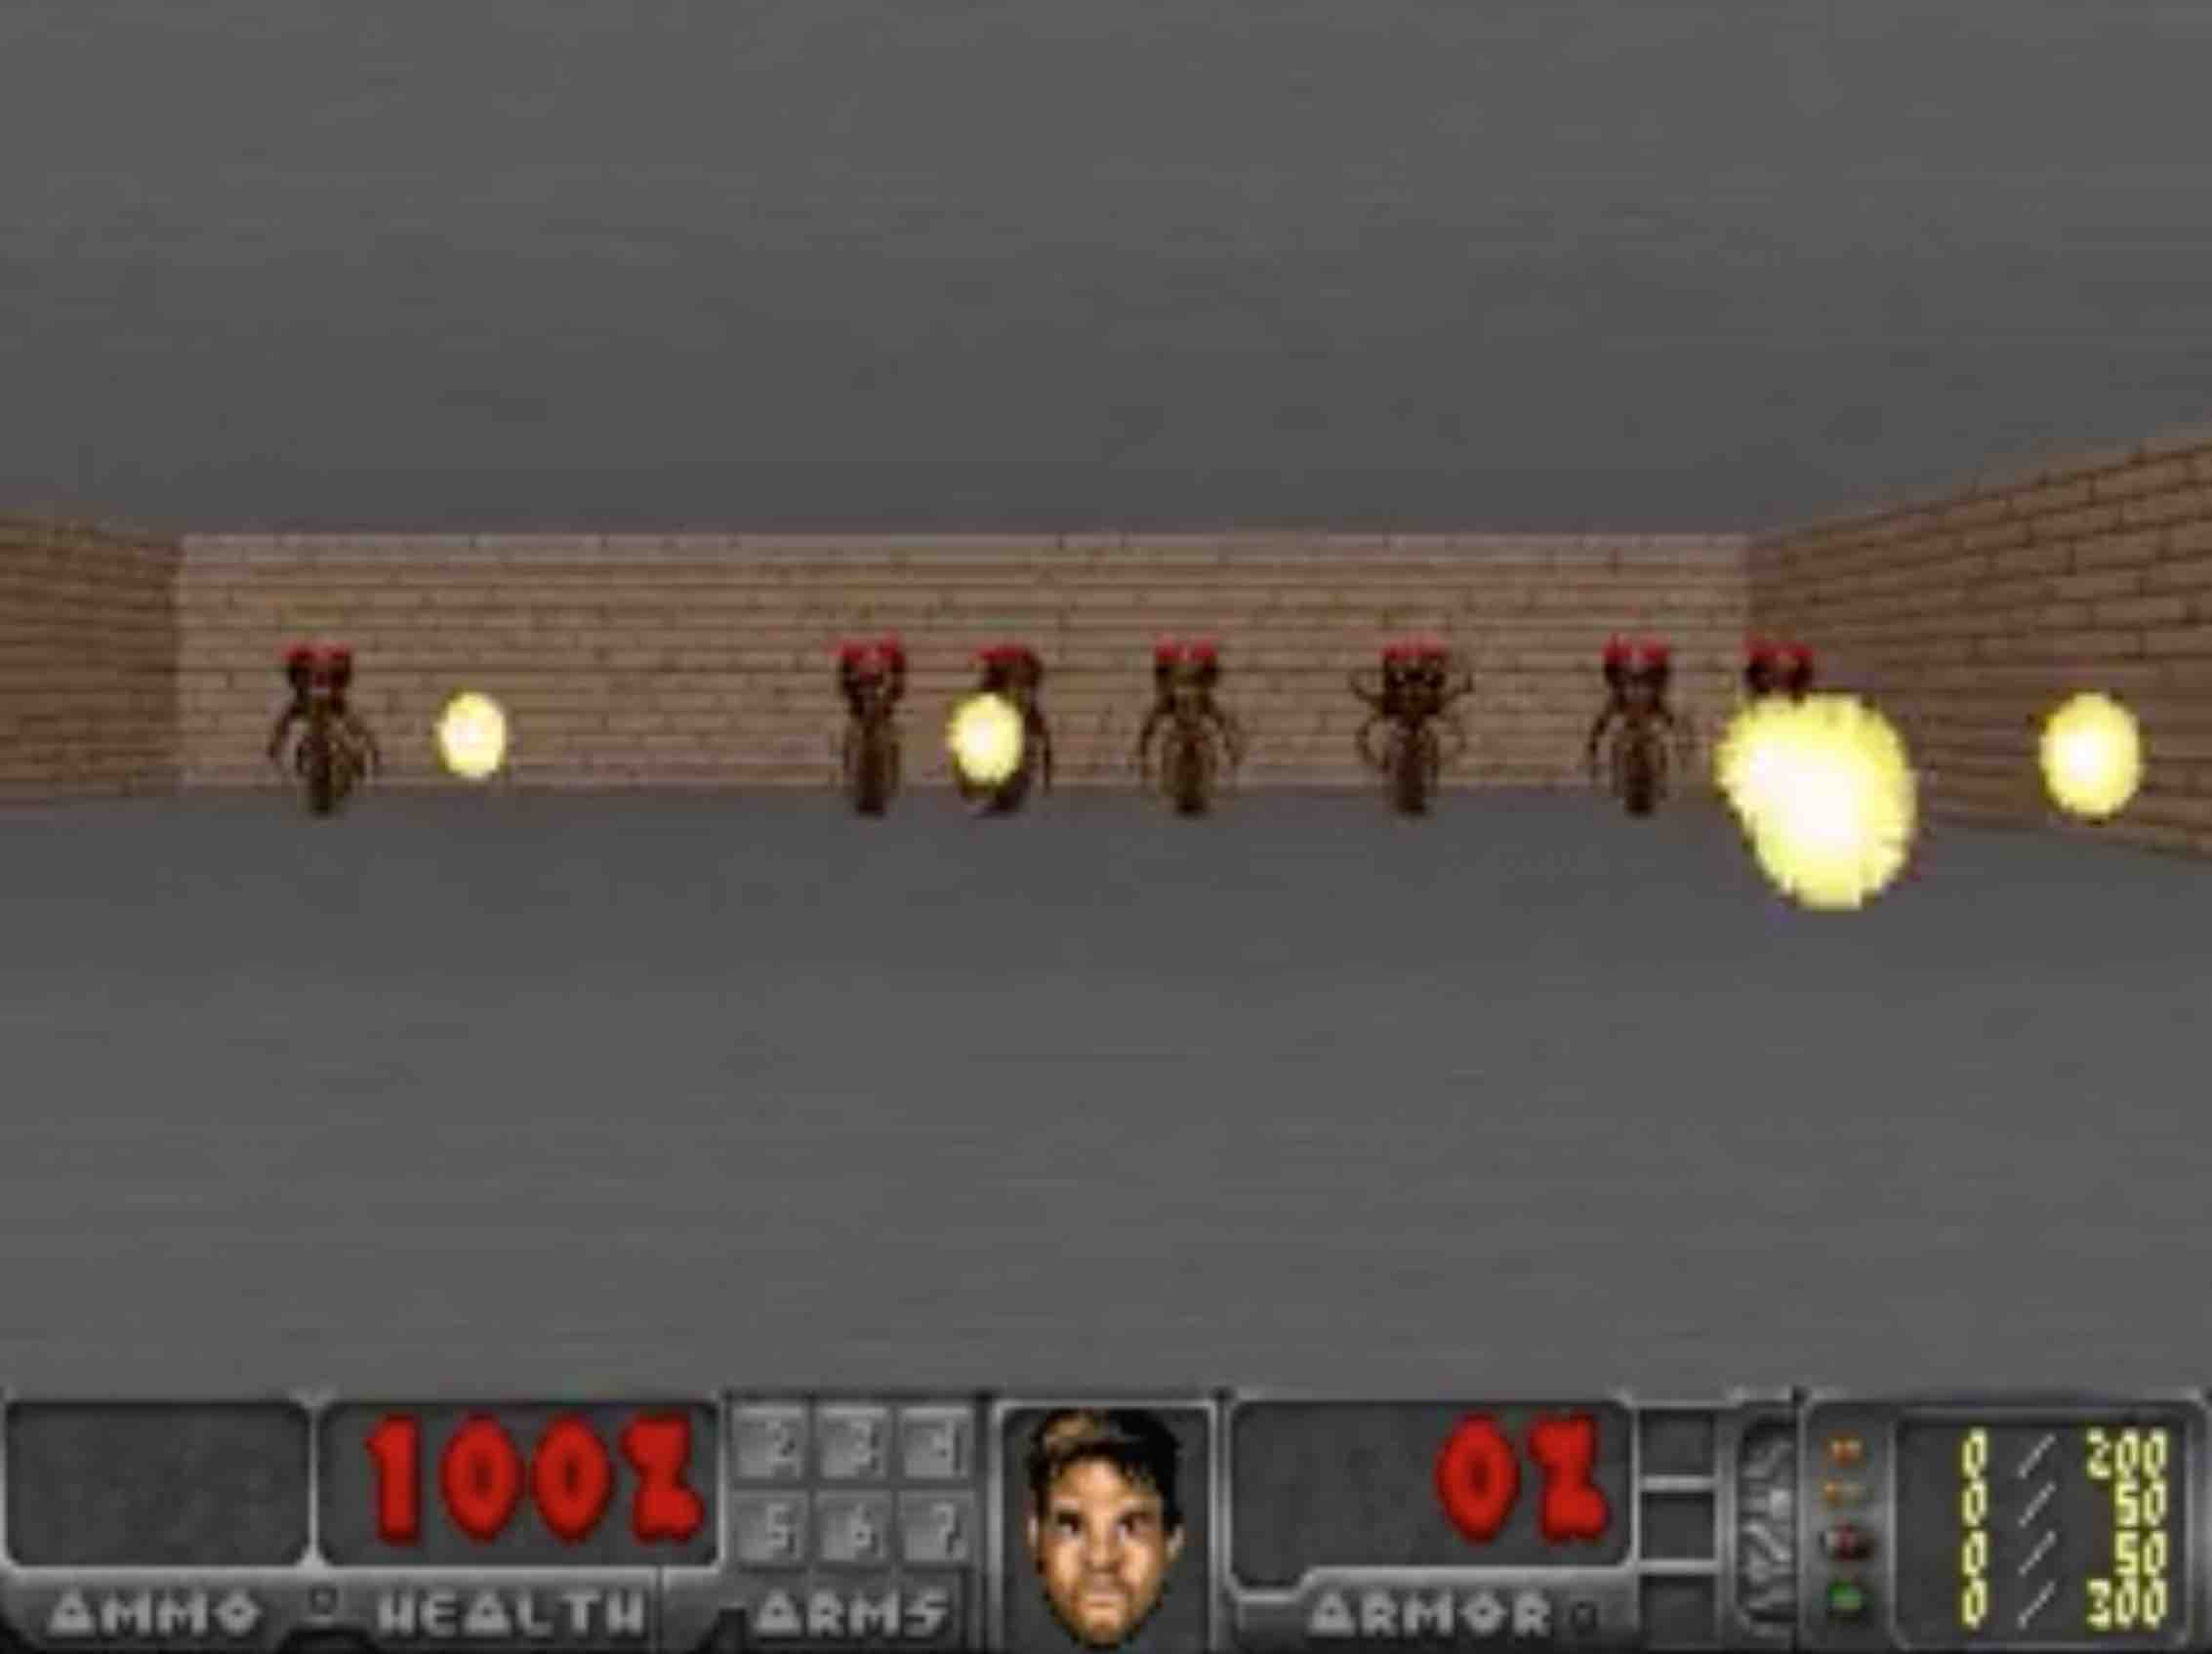
\includegraphics[width=0.23\textwidth]{images/doom2.jpeg}
	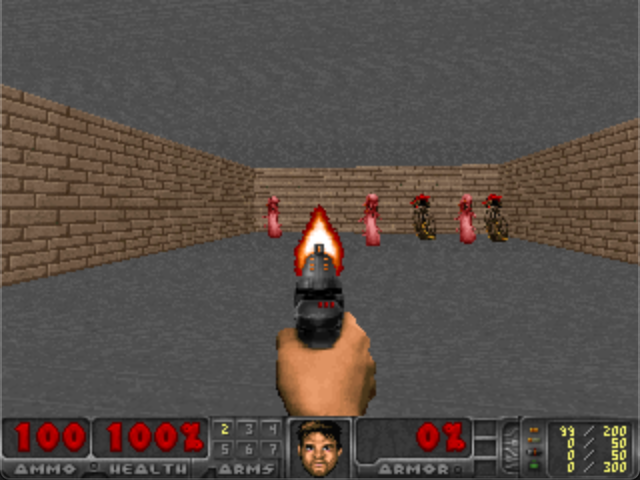
\includegraphics[width=0.23\textwidth]{images/doom1.png}
	\caption{The take_cover (left) and defend_the_line (right) scenarios}\label{fig:doom}
\end{figure}

The scenarios in ViZDoom~\cite{kempka2016vizdoom} are discrete action-space environments where the agent's goal is to survive in a room of monsters. The \texttt{take\_cover} scenario (left of \cref{fig:doom}) requires the agent to select between moving left or right to avoid fireballs launched towards the agent by opposing monsters. The agent receives a reward of $+1$ at every time step where the episode continues until the agent loses all of its health from being hit by fireballs. In the \texttt{defend\_the\_line} environment (right of \cref{fig:doom}), the agent selects between turning left, right or shooting a pistol with limited ammunition straight ahead with the goal of eliminating as many approaching monsters in order to survive. The agent receives $+1$ for each monster eliminated and $-1$ for losing all health from monster attacks.


\section{DEEP RL WITH WORLD MODELS}\label{approach}

In this section, we reintroduce the World Models architecture \cite{ha2018recurrent} in the context of reinforcement learning. A trained World Model can be incorporated in the RL training loop as shown in \cref{fig:worldmodel} to transform an image observation into a compressed representation that is then passed to the agent. This output consists of a latent encoding $z_t$ of the image from a VAE and the hidden state $h_t$ from a Gaussian Mixture Density RNN (MDRNN). The concatenation of these two vectors becomes the state feature representation, which the agent can treat as the environment's underlying state when learning an optimal policy.
\begin{figure}[h]
	\centering
	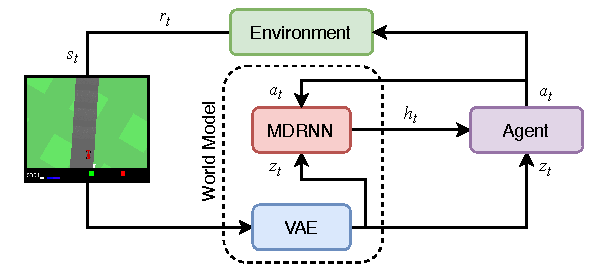
\includegraphics[width=0.49\textwidth]{images/worldmodel2.pdf}
	\caption{MDP Loop with a World Model}\label{fig:worldmodel}
\end{figure}

\subsection{VAE Model}

A VAE consists of an encoder network that compresses an input image $s_t$ into a latent feature vector $z_t$, and also a decoder network to reconstructed the image from the preserved features as shown in \cref{fig:vae}. The VAE parameterized by $\theta$ is trained to minimize the difference between the reconstructed image and the input image with the constraint of minimizing the KL divergence between the latent encoding space and the normal distribution which was found to suitable prior over the latent variable $z$ for maximum-likelihood feature representation~\cite{diederik2014auto}. This is achieved by minimizing the following loss function: 
\begin{equation}
    L_{\mathrm{VAE}}(s_t;\theta) = (s_t - \hat{s_t})^2 + D_{\mathrm{KL}}(p(z_t \mid s_t)\,\|\,\mathcal{N}(0,1)),
\end{equation}
where the first term minimizes the difference between the reconstructed and input image and the second term penalizes large shifts in the conditional latent state distribution $p(z_t \mid s_t)$ from a unit normal. A VAE is ideal for this task as it learns to encode the most important sources of variation from the distribution of training images within a small linear vector. The KL divergence term ensures that the model is able to sufficiently represent less frequent states without overfitting to a particular region of the state space.
\begin{figure}[h]
	\centering
	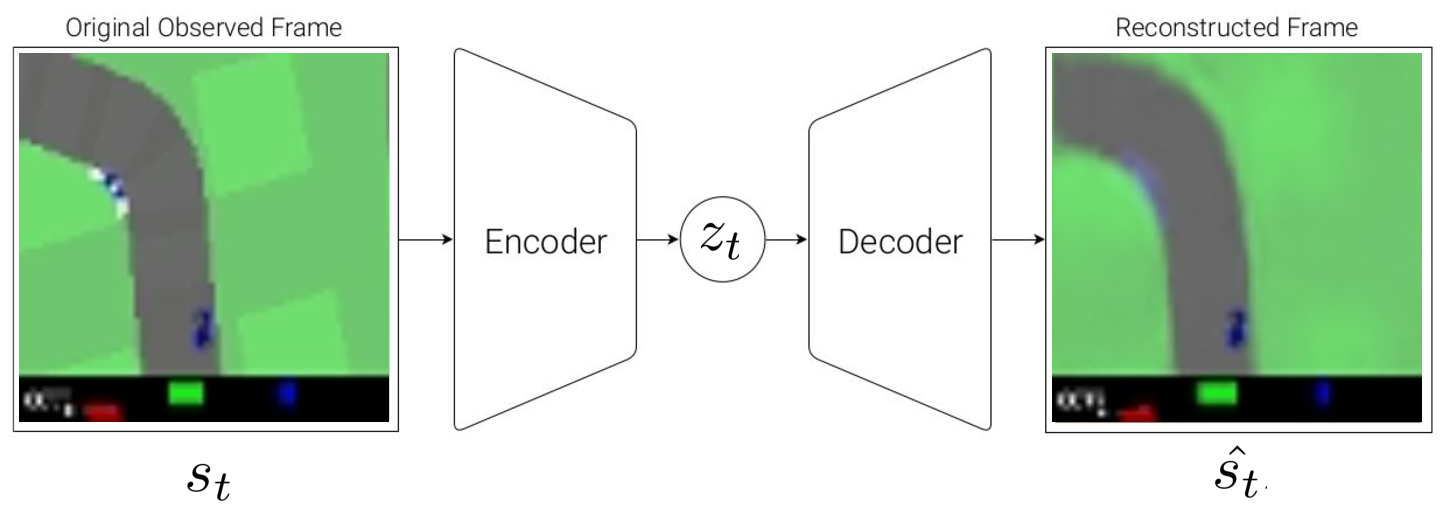
\includegraphics[width=0.49\textwidth]{images/vaes.pdf}
	\caption{Flow diagram of a VAE \cite{ha2018recurrent}}\label{fig:vae}
\end{figure}

\subsection{MDRNN Model}

While the VAE transforms a high-dimensional image into a low dimensional latent vector, it is only a static representation at a single point in time and lacks information about the temporal dynamics of the environment. Therefore, an RNN is trained to encode temporal information over a sequence of latent vectors. \Citeauthor{ha2018recurrent} utilized a Long-Short-Term-Memory (LSTM) to model the temporal changes in the next state through its hidden LSTM state $h_{t+1}$ calculated from the current latent vector $z_t$, chosen action $a_t$ and its current hidden state $h_t$~\cite{ha2018recurrent}. As the distribution of next states is often stochastic, the output of the LSTM is passed to a Gaussian-Mixture Density Network (MDN) \cite{bishop1994mixture} represented in \cref{fig:mdrnn} as a linear layer which outputs the mean $(\mu)$, standard deviation $(\sigma)$, and mixing weights $(\textbf{w})$, for a specified number of Gaussian distributions. The predicted next latent state can be sampled by first sampling a Gaussian index from the mixture weights $w$ and then sampling the latent vector $\hat{z}_{t+1}$ from the selected Gaussian. 
\begin{figure}[h]
	\centering
	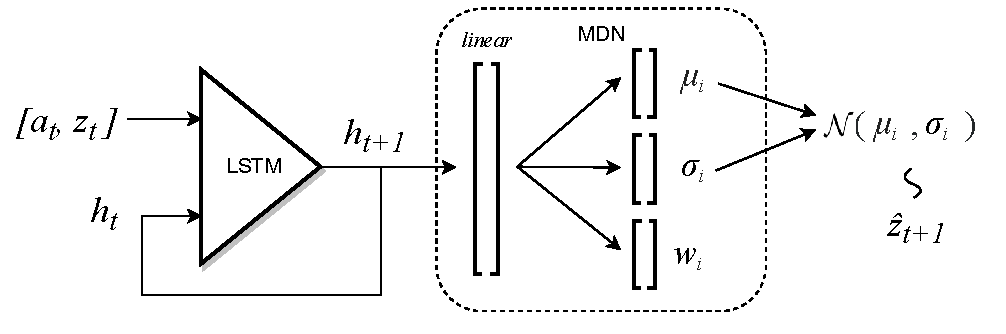
\includegraphics[width=0.5\textwidth]{images/MDRNN2.pdf}
	\caption{Flow diagram of a MDRNN}\label{fig:mdrnn}
\end{figure}

The MDRNN can be modeled as a function parameterized by $\beta$ defined as $ M(a_t,z_t;h_t;\beta) \rightarrow h_{t+1}, \hat{z}_{t+1},$ where $z$ is sampled from $\mathcal{N}(\mu_i, \sigma_i)$, and $i$ is sampled from a categorical distribution with probabilities \textbf{w} \cite{ellefsen2019mixture}. Given an experience tuple $(s_t, a_t, s_{t+1}, r_t, d_t)$, the latent states $z_t$ and $z_{t+1}$ can be obtained as the output of a trained VAE given inputs $s_t$ and $s_{t+1}$. Then, with the probability $p(z_{t+1} \mid \mu,\sigma;\beta)$ of sampling $z_{t+1}$ from $\mu$ and $\sigma$, the MDRNN $M$ can be trained by minimizing the following loss function:
\begin{dmath}
	L_{\mathrm{MDRNN}}(\beta) = -\mathbb{E}_{(z,z') \sim \mathrm{VAE}(\mathcal{E}),\ a \sim \mathcal{A},\ (\mu,\sigma,w) \sim M(a,z)} \\ \left[ \log \left( \sum^n_i w_i \ p(z' | \mu_i,\sigma_i;\beta) \right) \right] 
\end{dmath} 

\subsection{Controller Model}\label{sec:ctrl}

The controller model is a simple linear mapping of the latent state from the World Model to an action. It was noted in \cite{ha2018recurrent} that the hidden state of the MDRNN $h_t$ was sufficient for encoding temporal information of the current state since it is used to predict $\hat{z}_{t+1}$ from $z_t$ and $a_t$. As a result, the controller can be represented as a linear function $a_t = W_c \cdot [z_t, h_t] + b_c$ where $W_c$ is the weight and $b_c$ is the bias for the single-layer network. As the controller is designed to have the minimum number of parameters for a linear function of $[z_t, h_t]$, it can be optimized with the CMA-ES algorithm. In this paper, the controller is not considered part of the World Model, but instead as a baseline agent for benchmarking deep RL agents trained with the World Model.

\subsection{Training The World Model}

Since the variation in the image observation space is stationary over time for a fixed policy, this allows the VAE to be trained independently from the MDRNN. Similarly, as the controller is responsible only for policy optimization, it can be trained with simplified states from a pre-trained World Model. \cref{alg:wm} outlines the procedure for training each component of the World Model. Upon initializing the parameters of the VAE $V$, MDRNN $M$, and Controller $C$ with the appropriate \textsc{InitParameters} function, a dataset $\mathcal{D}$ is extended with $N$ trajectories sampled from the environment $\mathcal{E}$ using $C$ as the policy. Then, with learning rate $\alpha$, $V$ is trained on batches of images from $\mathcal{D}$. $M$ can then be trained using the previously trained $V$ to compress images to latent vectors. $C$ is then optimized using \textsc{CMA-ES} given a trained World Model ($V$,$M$). It is possible that one iteration of this training process is not enough to encounter optimal states of the environment since the initial trajectories are sampled with a random controller. Hence, this loop is repeated using the previously trained controller and World Model for a specified $S$ iterations depending on the complexity of the environment.

\section{DEEP RL WITH WORLD MODELS}

This section describes the process of training RL agents using a trained World Model, as well as the architecture of the RL algorithms to be trained with the World Model.

\subsection{Training RL Agents With The World Model}

Given a pre-trained World Model as the output from \cref{alg:wm}, the RL agent can focus solely on identifying the optimal mapping from latent features to actions that maximize total reward. \cref{alg:rl} describes the procedure for stepping through the environment $\mathcal{E}$ with a World Model consisting of the VAE $V$ and MDRNN $M$ that are either trained using \cref{alg:wm} or loaded from a previously trained World Model on the same environment $\mathcal{E}$. Then, the training of an RL policy $\pi$ towards an optimal policy occurs over a specified number of training trajectories. At the start of each training trajectory, the MDRNN hidden state $h$ is initialized with \textsc{InitHidden}, the initial observation $s$ is sampled from the environment with \textsc{InitState}, and the latent encoding $z$ of the initial image observation is sampled from the VAE. The flag $d$ signifying reaching a terminal state is initialized to false. Then, until a terminal state is reached, the RL training loop proceeds with the \textsc{Step} function applying each agent action $a$ to the environment and outputting the next observation $s'$, reward $r$ and updated terminal flag $d$. The observations $s$ and $s'$ are replaced with the latent state $[z,h]$ and next latent state $[z',h']$, where $z$ and $h$ are the outputs of the VAE $V$ and MDRNN $M$ respectively. The agent is then given the updated experience tuple with latent states using the where it can store or use in a training update through the \textsc{Train} function implemented according to a specified RL algorithm.

\begin{algorithm}[t]
   % \SetAlgoLined
    \caption{Training Loop for World Model}\label{alg:wm}
    \begin{algorithmic}[1] 
        \Procedure{TrainWorldModel}{$\mathcal{E}, S, N$} 
            \State $ V(s;\theta) \gets \Call{InitParameters}{\theta} $
            \State $ M(z,a;\beta) \gets \Call{InitParameters}{\beta} $
		    \State $ C(z,h;W_c, b_c) \gets \Call{InitParameters}{W_c, b_c} $
		    \State $ \mathcal{D} \gets \emptyset $
            \For{$ i \textbf{ in } \{1, \ldots, S\}$} 
                \State $\mathcal{D} \gets \mathcal{D} \cup \Call{SampleTrajectories}{\mathcal{E},C,N}$
                \For{$ batch $ $\textbf{in}$ $\mathcal{D}$}
    				\State $ \mathcal{L}_{\theta} \gets L_{\mathrm{VAE}}(batch;\theta) $
    				\State $ \theta \gets \theta - \alpha \nabla \mathcal{L}_{\theta}$
			    \EndFor
                \For{$ batch $ $\textbf{in}$ $\mathcal{D}$}
    				\State $ \mathcal{L}_{\beta} \gets L_{\mathrm{MDRNN}}(V,batch;\beta) $
				    \State $ \beta \gets \beta - \alpha \nabla \mathcal{L}_{\beta}$
			    \EndFor
			    \State $ C \gets \Call{CMA_ES}{C,V,M} $
            \EndFor
            \State \textbf{return} $V, M$
        \EndProcedure
    \end{algorithmic}
\end{algorithm}

\begin{algorithm}[t]
    %\SetAlgoLined
    \caption{RL Training With Trained World Model}\label{alg:rl}
    \begin{algorithmic}[1] 
        \Procedure{TrainRLAgent}{$\mathcal{E}, S, N$} 
            \State $ V, M \gets \Call{TrainWorldModel}{\mathcal{E}, S, N} $
            \State $ \pi(z,h;$\textbf{$\phi$}$) \gets \Call{InitParameters}{\phi} $
            \For{$ \textrm{each trajectory} $ $\textbf{do}$} 
                \State $ h \gets \Call{InitHidden}{M} $
    			\State $ s \gets \Call{InitState}{\mathcal{E}} $
    			\State $ z \gets V(s;\theta) $
    			\State $ d \gets $ false
    			\While{$ d =$ false}
    			    \State $ a \gets \pi([z,h];\phi) $
    				\State $ s', r, d \gets \Call{Step}{\mathcal{E}, a}$
    				\State $ h' \gets M(z,a;h;\beta) $
    				\State $ z' \gets V(s';\theta) $
    				\State $ \Call{Train}{\pi, ([z,h], a, [z',h'], r, d)} $
    				\State $ [z,h] \gets [z',h'] $
    			\EndWhile
            \EndFor
        \EndProcedure
    \end{algorithmic}
\end{algorithm}

\begin{figure*}[ht!]
	\centering
    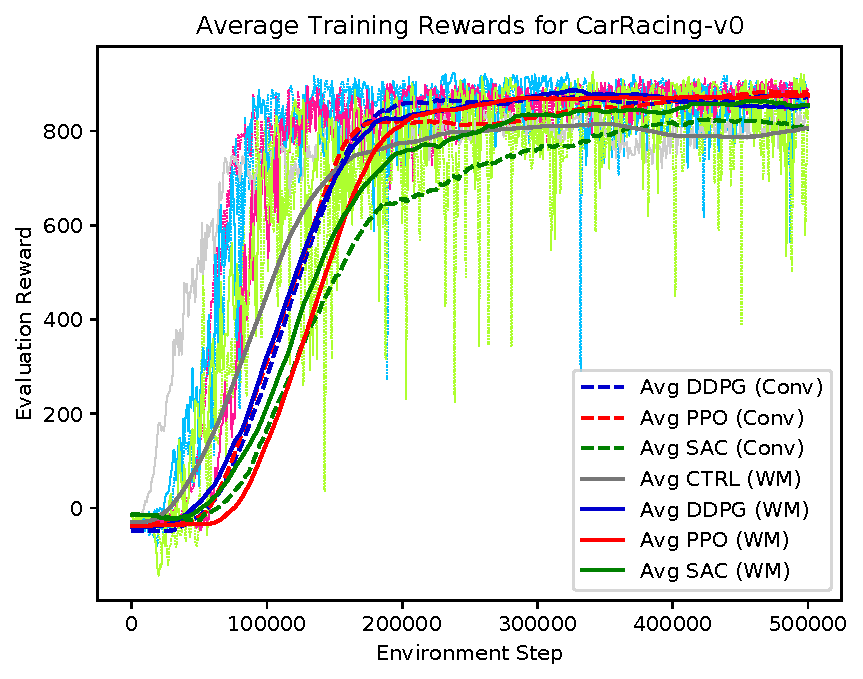
\includegraphics[width=0.325\linewidth]{images/CarRacing-v0.pdf}
    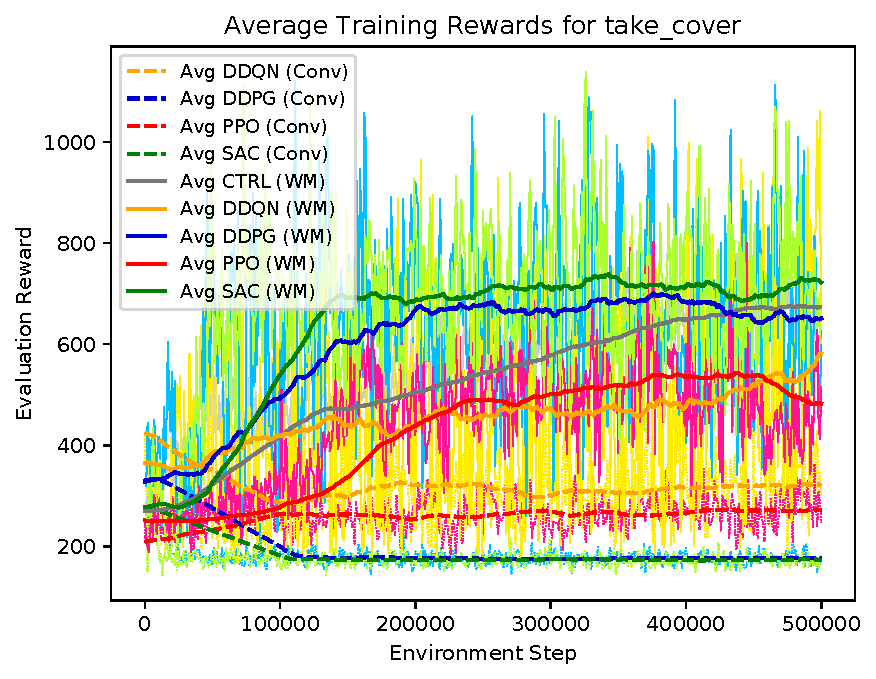
\includegraphics[width=0.33\linewidth]{images/take_cover.pdf}
    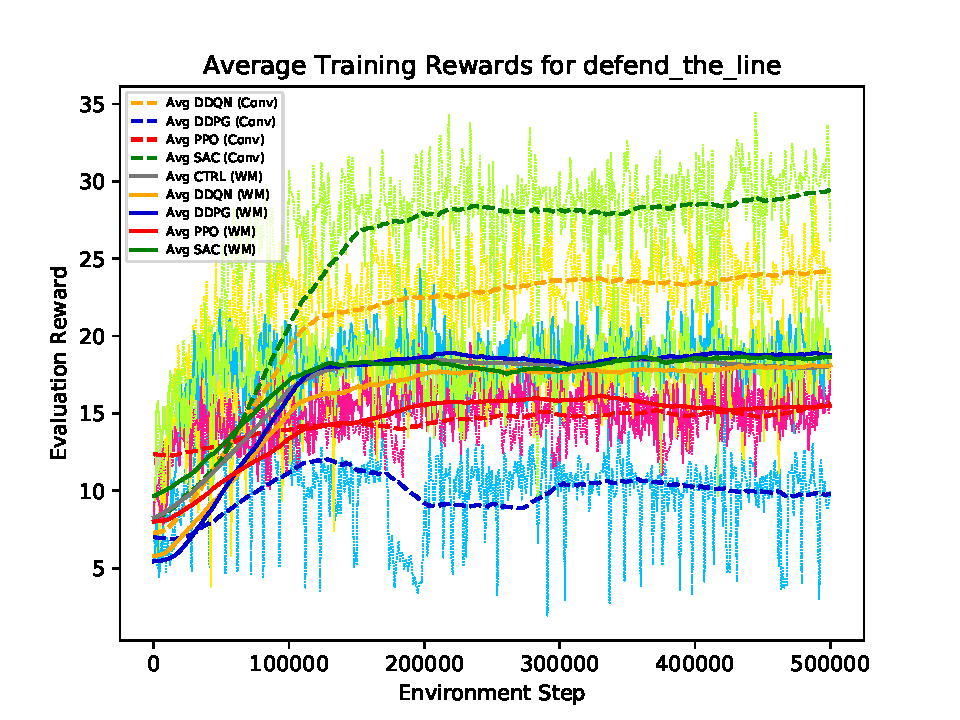
\includegraphics[width=0.32\linewidth]{images/defend_the_line.pdf}
    \caption{The rolling average evaluation rewards over the previous $100000$ steps for different RL algorithms trained in the CarRacing-v0 (left), take_cover (mid), and defend_the_line (right) environments. In each plot, the solid thick lines represent training with the pre-trained World Model and dashed thick lines represent training using convolutional layers. The thin lines represent evaluation rewards every $1000$ steps.}\label{fig:res}
\end{figure*}

\subsection{RL Agent Architecture}

The RL algorithms to be trained with the World Model include Double DQN (DDQN)~\cite{wang2015dueling}, DDPG~\cite{lillicrap2015continuous}, PPO~\cite{schulman2017proximal}, and SAC~\cite{haarnoja2018soft}. These agents will be tested first with raw grey-scale image inputs to evaluate the baseline performance of learning an environment representation along with the learning of the optimal policy. For the baseline, each state input will consist of the current image observation stacked on top of the two previous observations. Then, the architecture of the baseline actor and critic will consist of a convolutional component to reduce the 2D image to a 1D vector which is then passed to a feed-forward component which will output the desired action or state-value. The convolutional component will share the same network architecture as the VAE encoder having four convolutional layers. The feed-forward component will consist of three layers to map the output of the convolutional component or world model to the desired output size of the actor or critic.

All agents will be trained on batches of experience tuples from $16$ parallel environments as done in~\cite{mnih2016asynchronous}. An experience replay buffer of a maximum size $100000$ samples will be used for off-policy algorithms DDQN, DDPG and SAC. DDQN and DDPG rely on explicit random exploration schedules which will be implemented with a Brownian noise process where the scale of noise is reduced from $1.0$ to a minimum of $0.02$ at a decay rate of $0.98$ after each trajectory.\footnote{The complete implementation is available on Github at https://github.com/sisl/WorldModelsForDeepRL} %https://github.com/shawnmanuel000/WorldModelsForDeepRL}
\section{EXPERIMENTAL SETUP}\label{experiments}

To evaluate the effectiveness of the World Model, we trained each RL algorithm for $500000$ steps on each of the three environments (except DDQN on \texttt{CarRacing-v0} due to continuous state space) with and without the World Model. The World Model was trained over two iterations for each component with $1000$ sampled trajectories added to the data set at each iteration, where the controller was trained for $500$ generations using CMA-ES. The training plots in \cref{fig:res} show the variability in the effect of the World Model on training efficiency. For most RL algorithms, training with the World Model outperformed the controller trained using CMA-ES in terms of maximum average reward.

The results for the \texttt{CarRacing-v0} environment in \cref{fig:res} (left) show that agents trained with the World Model appeared to achieve the same overall performance as agents trained using a convolutional network with stacked images. Although training PPO and DDPG without the World Model were able to achieve faster improvement in average reward, the agents trained using the World Model were able to maintain this performance with less variation in rewards at each training iteration. The time required to train agents with the World Model was significantly less, taking approximately 7 hours in contrast to the 11 hours required to train a new convolutional network for each agent.

The \texttt{take\_cover} environment rewards shown in \cref{fig:res} (middle) exhibit the most variation between agents using the Model and those without. It is clear that only the agents trained with the World Model were able to improve their average score while the agents training a convolutional network collapsed to a degenarate policy. Investigating playbacks of the trained agents revealed that policies converged to only move left. \Citeauthor{ha2018recurrent} referred to this being the result of the credit assignment problem where backpropagation of gradients through a large neural network with many layers and parameters can hinder convergence~\cite{ha2018recurrent}. However, the World Model enables the agent to use a shallower network for policy learning.

In the \texttt{defend_the_line} environment, training with the world model achieved a constant but stable reward compared to the agents using convolutional networks as seen in \cref{fig:res} (right). However, an outlying observation of SAC and DDQN converging to a much higher average reward when trained without a World Model suggests that the World Model may not always capture the optimal variational features for optimization of the policy for fine variations in the image states. To address this issue, the pre-trained World Model could be further trained along with the policy to allow for finer optimization at the image processing level.

As the plots show, the World Model has many benefits for deep RL. We demonstrated that a single pre-trained World Model can generalize the environment representation for use with different agents learning in the same environment, which can be applied to various domains with a stationary state distribution. It reduces the number of parameters that the RL agent needs to update, which reduces the time taken for each update, equivalently leading to faster training. Along with saving time, the World Model reduces the memory requirement of off-policy agents using a replay buffer where high dimensional states can be directly mapped to a latent state with the World Model before being stored.

\section{CONCLUSION}

In this paper, we applied the recent World Models architecture to the field of deep reinforcement learning to simplify a high dimensional image state into a compressed feature vector for a reinforcement learning agent to learn an optimal policy. We focused on training two algorithms, DDPG and PPO, on OpenAI Gym's \texttt{CarRacing-v0} environment. It was found that the World Model significantly improved the stability of the PPO algorithm, allowing it to achieve an average score of 812 using the World Model compared to 153 without it. The DDPG algorithm achieved an average score of 842 with the World Model with a standard deviation of less than half of that without the World Model. Overall, our approach achieved the highest average score for the DDPG and PPO algorithm compared to previous approaches without having to simplify the continuous action space.

Future work could focus on addressing the credit assignment problem prevalent in reinforcement learning by incorporating generalized exploration schemes or adjusting the hyperparameters based on approaches for solving similarly complex environments. Another direction is to improve the accuracy of the World Model with attention mechanisms, or allowing the World Model to be optimized during policy optimization. Overall, we found that the World Model architecture has potential to improve stability and speed up the training of reinforcement learning agents in complex high dimensional environments, along with reducing the required size of the policy.

% \bibliography{paper}
% \bibliographystyle{IEEEtran}
\renewcommand*{\bibfont}{\small}
\printbibliography


\end{document}
